% =====================================================================
% APÊNDICE C -- curvas de SER dos três grupos (2026-11-09, pedido da autora: todas aqui
% por enquanto; ela escolhe depois quais voltam para os Resultados). Texto e figuras vieram
% das subseções "Curvas de SER" de chapters/RESULTADOS/formatos.tex.
% =====================================================================

% 2026-11-09: o grupo 1 (texto e figuras) voltou para os Resultados (sec:resultados-curvas),
%   a pedido da autora. Aqui ficam os grupos 2 e 3.
% 2026-11-10: as curvas do grupo 1 com os três formatos voltaram para cá; nos Resultados
%   ficam só o <18,8> e o <24,12> (curvas_ser_G1_<mod>_2fmt.pdf).
\textcolor{red}{Cada grupo tem uma figura por modulação. As colunas são os formatos escolhidos do grupo (Tabela~\ref{tab:formatos-escolhidos}), e, na primeira coluna, a faixa só tem as configurações de IoTh de 10~dB. As linhas são as condições de teste, escolhidas como nos Resultados (Seção~\ref{sec:resultados-curvas}).}

\section{\texorpdfstring{\textcolor{red}{Grupo 1: $M = 128$, $C = 8$}}{Grupo 1: M = 128, C = 8}}\label{subsubsec:curvas-grupo1}
\textcolor{red}{As Figuras~\ref{fig:curvas-g1-16qam-completa} e \ref{fig:curvas-g1-qpsk-completa} acrescentam o $\langle 26,12\rangle$ às curvas do grupo 1. Com as duas modulações, ele fica muito perto do $\langle 24,12\rangle$.}

\begin{figure}[!ht]
\caption{\textcolor{red}{Curvas de SER no grupo 1 com 16-QAM, configurações 1A, 1B, 1E e 1F, em todos os formatos escolhidos.}}
\label{fig:curvas-g1-16qam-completa}
\vspace{4pt} % a classe zera o espaço entre a caption e a figura
\centering
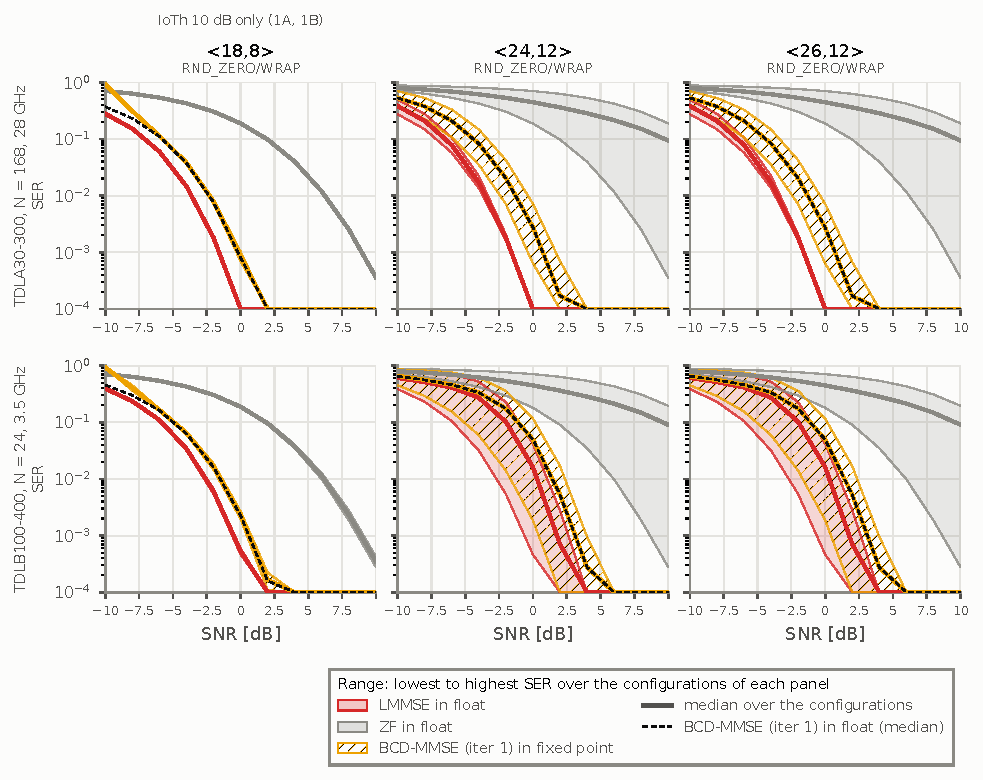
\includegraphics[width=\textwidth]{Images/RESULTADOS/curvas_ser_G1_16qam.pdf}
\vspace{4pt}
\legend{\textcolor{red}{Fonte: a autora.}}
\end{figure}

\begin{figure}[!ht]
\caption{\textcolor{red}{Curvas de SER no grupo 1 com QPSK, configurações 1C, 1D, 1G e 1H, em todos os formatos escolhidos.}}
\label{fig:curvas-g1-qpsk-completa}
\vspace{4pt} % a classe zera o espaço entre a caption e a figura
\centering
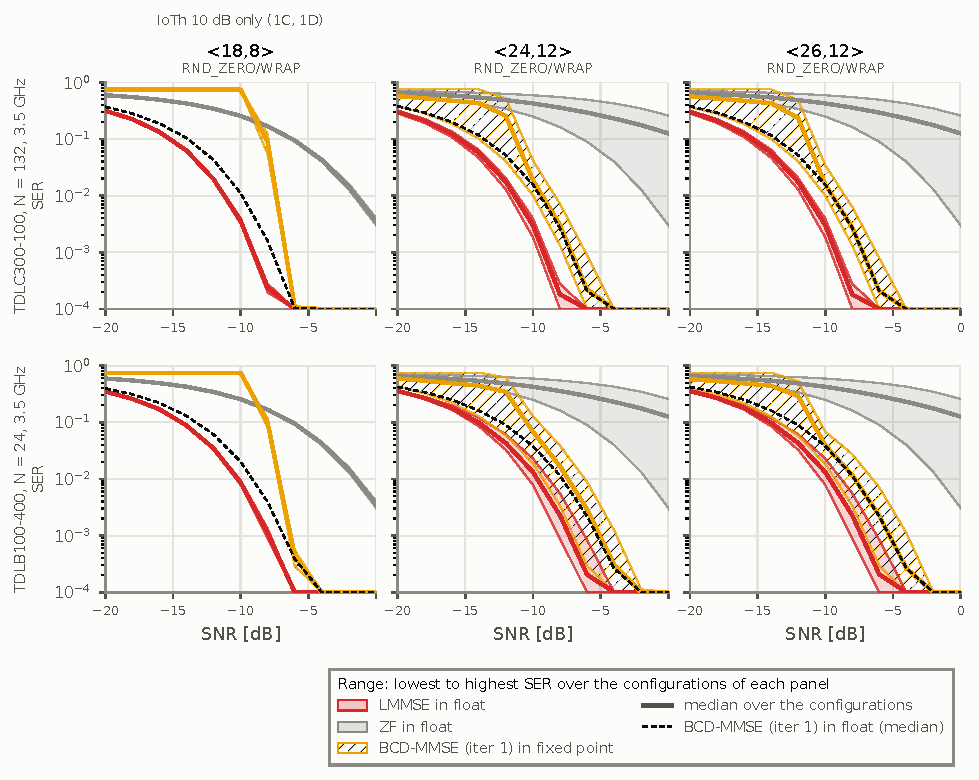
\includegraphics[width=\textwidth]{Images/RESULTADOS/curvas_ser_G1_qpsk.pdf}
\vspace{4pt}
\legend{\textcolor{red}{Fonte: a autora.}}
\end{figure}

\section{\texorpdfstring{\textcolor{red}{Grupo 2: $M = 256$, $C = 8$}}{Grupo 2: M = 256, C = 8}}\label{subsubsec:curvas-grupo2}
\textcolor{red}{Nas Figuras~\ref{fig:curvas-g2} e \ref{fig:curvas-g2-qpsk}, com 16-QAM, os formatos ficam muito perto do ponto flutuante, e o ponto flutuante fica muito perto do LMMSE. Como no grupo 1, a TDLB100-400 tem a maior diferença entre as curvas das configurações. Com QPSK, o $\langle 28,14\rangle$ ainda se afasta um pouco do ponto flutuante, e o $\langle 30,14\rangle$ fica perto dele.}

\begin{figure}[!ht]
\caption{\textcolor{red}{Curvas de SER no grupo 2 com 16-QAM, configurações 2A, 2B, 2E e 2F.}}
\label{fig:curvas-g2}
\vspace{4pt} % a classe zera o espaço entre a caption e a figura
\centering
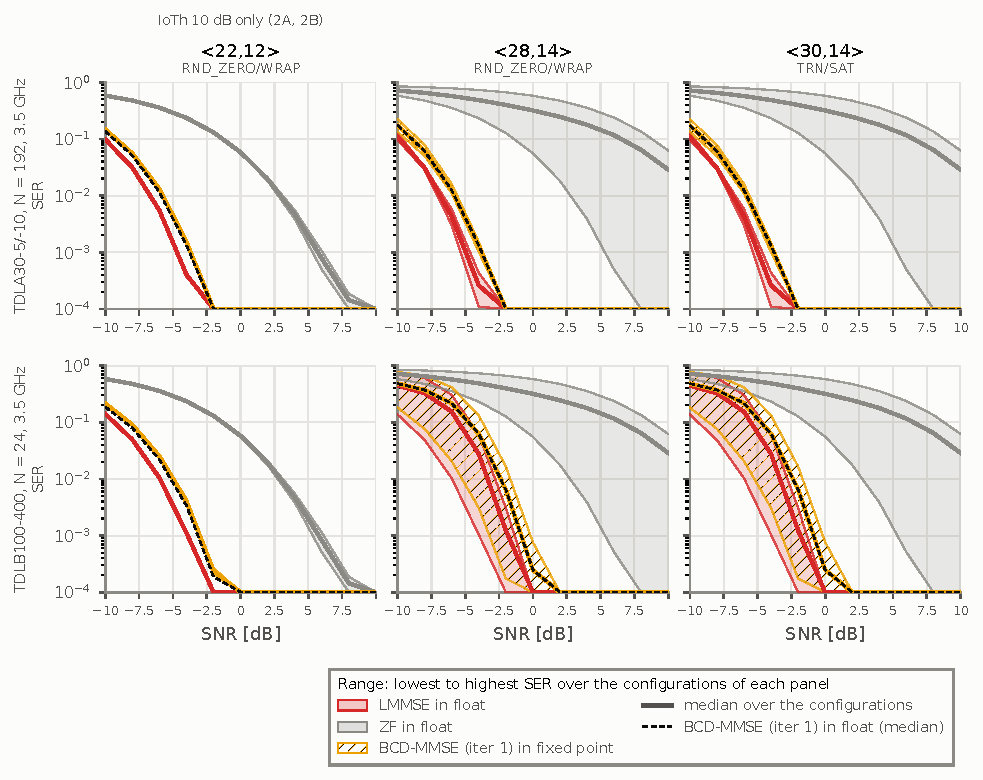
\includegraphics[width=\textwidth]{Images/RESULTADOS/curvas_ser_G2_16qam.pdf}
\vspace{4pt}
\legend{\textcolor{red}{Fonte: a autora.}}
\end{figure}

\begin{figure}[!ht]
\caption{\textcolor{red}{Curvas de SER no grupo 2 com QPSK, configurações 2C, 2D, 2G e 2H.}}
\label{fig:curvas-g2-qpsk}
\vspace{4pt} % a classe zera o espaço entre a caption e a figura
\centering
% ponto fixo da grade inteira (modo_fixo_3dB_qpsk_256), desde -20 dB
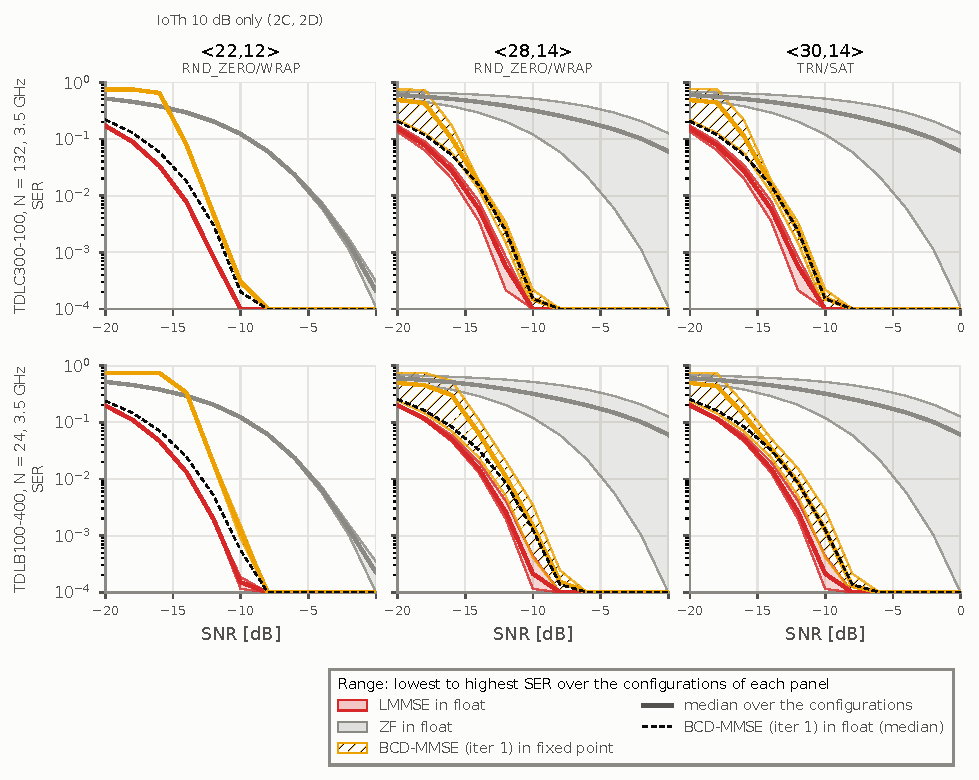
\includegraphics[width=\textwidth]{Images/RESULTADOS/curvas_ser_G2_qpsk.pdf}
\vspace{4pt}
\legend{\textcolor{red}{Fonte: a autora.}}
\end{figure}

\section{\texorpdfstring{\textcolor{red}{Grupo 3: $M = 256$, $C = 16$}}{Grupo 3: M = 256, C = 16}}\label{subsubsec:curvas-grupo3}
\textcolor{red}{Na Figura~\ref{fig:curvas-g3}, com 16-QAM, o grupo 3 fica entre os grupos 1 e 2, tanto no SNR necessário quanto na diferença entre as configurações. Na Figura~\ref{fig:curvas-g3-qpsk}, com QPSK, o $\langle 24,12\rangle$ se afasta do ponto flutuante, e o $\langle 30,14\rangle$ fica perto dele.}

\begin{figure}[!ht]
\caption{\textcolor{red}{Curvas de SER no grupo 3 com 16-QAM, configurações 3A, 3B, 3E e 3F.}}
\label{fig:curvas-g3}
\vspace{4pt} % a classe zera o espaço entre a caption e a figura
\centering
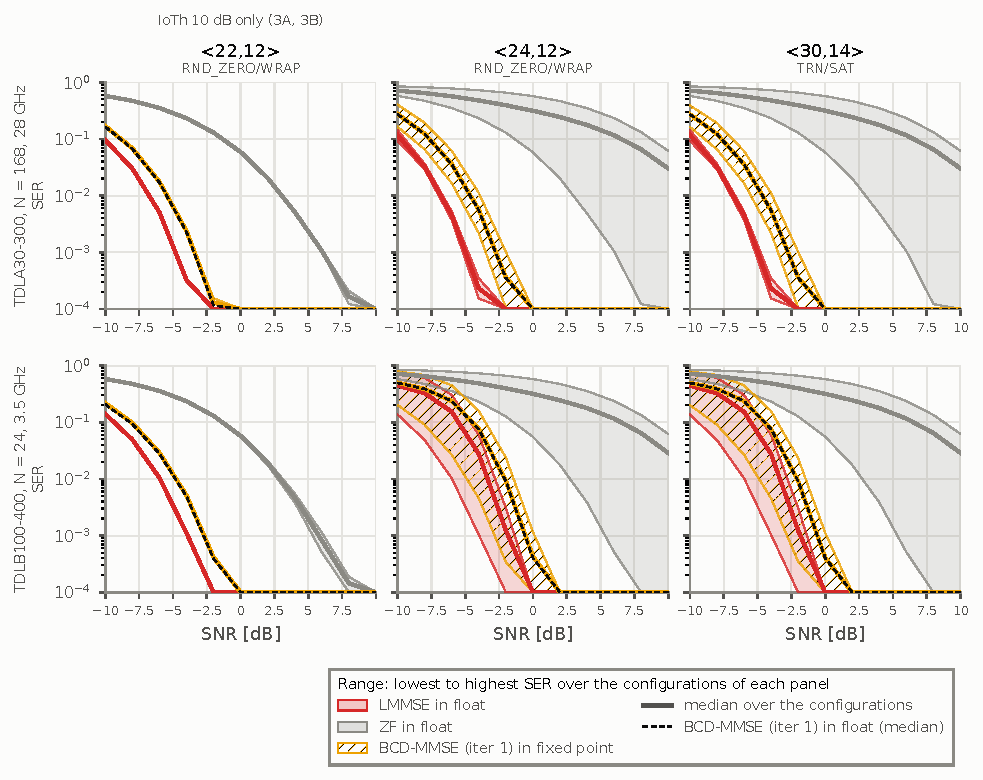
\includegraphics[width=\textwidth]{Images/RESULTADOS/curvas_ser_G3_16qam.pdf}
\vspace{4pt}
\legend{\textcolor{red}{Fonte: a autora.}}
\end{figure}

\begin{figure}[!ht]
\caption{\textcolor{red}{Curvas de SER no grupo 3 com QPSK, configurações 3C, 3D, 3G e 3H.}}
\label{fig:curvas-g3-qpsk}
\vspace{4pt} % a classe zera o espaço entre a caption e a figura
\centering
% ponto fixo da grade inteira (modo_fixo_3dB_qpsk_256), desde -20 dB
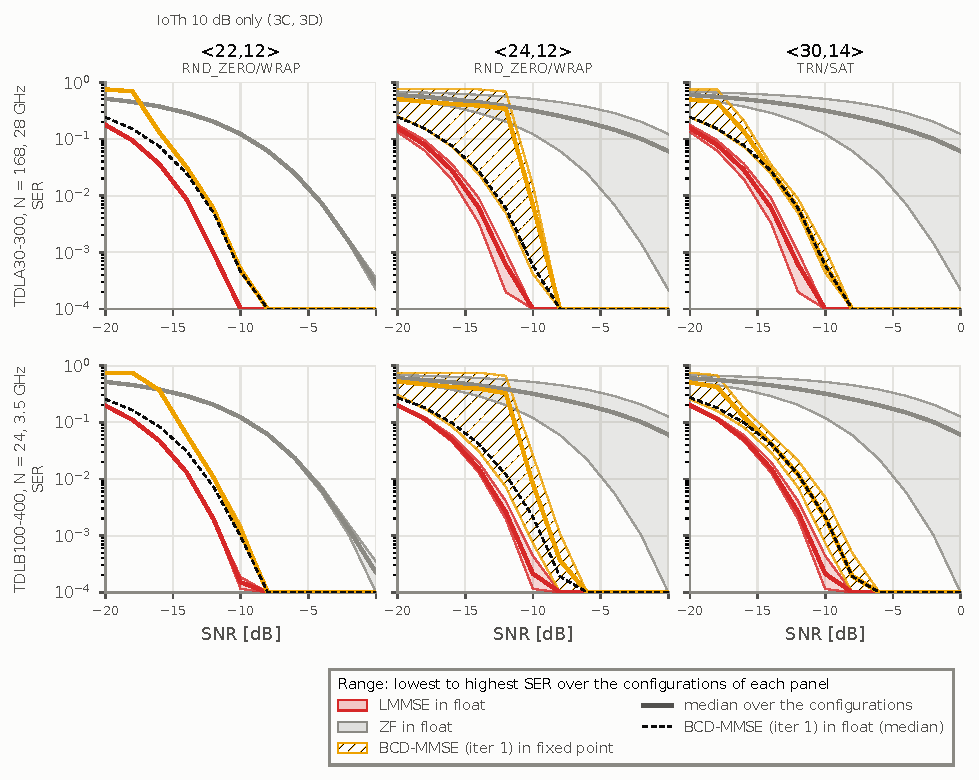
\includegraphics[width=\textwidth]{Images/RESULTADOS/curvas_ser_G3_qpsk.pdf}
\vspace{4pt}
\legend{\textcolor{red}{Fonte: a autora.}}
\end{figure}
